In this section I will look at similar work that I can use for my thesis. These works are not finished, so they are subject to change at any time.

\subsection{WebRTC to IMS}
There is an ongoing effort at the 3GPP on giving \gls{wrtc} clients access to \gls{ims} with 3GPP TR 23.701\cite{3gpp-wrtc-access-ims} as the current proposed architecture. \gls{ims} is basically an architectural framework for delivering IP multimedia services. It was originally designed for evolving mobile networks beyond \gls{gsm}. Later it has evolved to include Wireless LAN and fixed lines, it's intended to aid the access of multimedia and voice applications across different networks. This study is relevant because most telecom companies already have IMS or a similar architecture in place for doing real-time communication. The following diagram shows the proposed architecture:

\begin{figure}[here]
\centerline{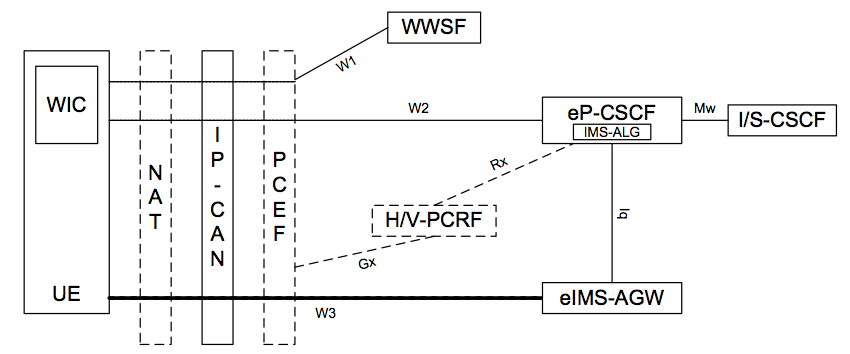
\includegraphics[scale=0.5]{3gpp-wrtc-ims-architecture.png}}
\caption{WebRTC IMS architecture by 3GPP TR 23.701.}
\label{fig:wrtc-ims-architecture}
\end{figure}

Let's look at the main elements:

\textbf{WebRTC IMS Client (WIC)}
is downloaded from the WWSF. It provides the application logic and \gls{wrtc} API calls to access the communication services of \gls{ims}. It works on any device supporting a browser that supports \gls{wrtc}.

\textbf{User Equipment(UE)}
is a device or application. It can be a web application running in a browser, a tablet or mobile phone.

\textbf{WebRTC Web Server Function (WWSF)}
is from where the client is downloaded. This could be a web server hosting the WIC, or an app store such as Google Play.

\textbf{P-CSCF enhanced for WebRTC (eP-CSCF)}
is the entry point of \gls{sip} requests. SIP is a protocol used for signaling, and they propose to receive SIP over WebSockets. It adapts signaling on the \gls{wrtc} side to standard IMS-SIP. The specification is open to the use of different protocols, but this is the proposed solution.

\textbf{IMS Access Gateway enhanced for WebRTC (eIMS-AGW)}
supports \gls{rtcweb} media as defined by \gls{ietf}. It needs to support these functions:
\begin{itemize}
\item{SRTP-DTLS. \gls{sdes} is what's used in \gls{ims}}
\item{Audio/video transcoding. H.264 is the \gls{ims} standard}
\item{RTCP demultiplexing. \gls{rtcweb} supports multiplexing of audio/video calls and RTP/RTCP over same RTP session and port. This is not supported in \gls{ims}, so this component needs to support demultiplexing.}
\end{itemize}

In addition this component must also support STUN connectivity checks.

\textbf{IP Connectivity Access Network (IP-CAN)}
is used to reach the IMS core from the UE. Can be LTE\footnote{Long-Term Evolution is a standard for wireless communication of high-speed data for mobile phones.} for mobile, DSL or WLAN.

\textbf{Policy and Charging Rules Function (PCRF) and Policy and Charging Enforcement Function (PCEF)}
supports policy and charging control decisions based on session and media-related information obtained from the P-CSCF. It uses deep packet inspection and decides based on rules whether the traffic is allowed or not.

\textbf{Network Address Translation (NAT)}
the WIC would normally be behind a NAT element, so a box has been included in the diagram.

\subsection{Doubango Telecom}
Doubango Telecom has created a Smart SIP and Media Gateway to connect WebRTC endpoints\footnote{http://webrtc2sip.org/}. It's called webrtc2sip and it uses RTCWeb and SIP technologies. It allows your browser to make and receive calls to and from any SIP endpoint. The gateway contains four modules: a SIP Proxy, a RTCWeb Breaker, a Media Coder, and a Click-to-Call service. The first three are relevant to integrating WebRTC with enterprise communications. The SIP Proxy converts the SIP transport from WebSockets to SIP over UDP or TCP, which is supported by most enterprise networks, and the RTCWeb Breaker make support for ICE and SRTP-DTLS when negotiating media streams between WebRTC and SIP endpoints. Lastly, the Media Coder will allow us to make calls between browsers and SIP endpoints supporting different codecs.